\documentclass[10pt, conference, compsocconf]{IEEEtran}

\usepackage{cite}
\usepackage[pdftex]{graphicx}
\usepackage[cmex10]{amsmath}
\usepackage{algorithmic}
\usepackage{array}

\usepackage{mdwmath}
\usepackage{mdwtab}


\usepackage{eqparbox}
\usepackage[caption=false,font=footnotesize]{subfig}
\usepackage{fixltx2e}
%\usepackage{stfloats}
\usepackage{url}
\usepackage{amssymb}
\usepackage{filecontents}
\usepackage{comment}
\usepackage{url}
\usepackage{balance}
\usepackage{booktabs}

% correct bad hyphenation here
\hyphenation{op-tical net-works semi-conduc-tor}


\begin{document}
%
% paper title
% can use linebreaks \\ within to get better formatting as desired
\title{On Speeding-up Parallel Jacobi Iterations for SVDs}


% author names and affiliations
% use a multiple column layout for up to two different
% affiliations

\author{\IEEEauthorblockN{Soumitra Pal \qquad Sudipta Pathak \qquad Sanguthevar Rajasekaran}
\IEEEauthorblockA{Computer Science and Engineering, University of Connecticut\\
371 Fairfield Road, Storrs, CT 06269, USA\\
\texttt{\small \em \{mitra@,sudipta.pathak@,rajasek@engr.\}uconn.edu}}}

% conference papers do not typically use \thanks and this command
% is locked out in conference mode. If really needed, such as for
% the acknowledgment of grants, issue a \IEEEoverridecommandlockouts
% after \documentclass

% for over three affiliations, or if they all won't fit within the width
% of the page, use this alternative format:
% 
%\author{\IEEEauthorblockN{Michael Shell\IEEEauthorrefmark{1},
%Homer Simpson\IEEEauthorrefmark{2},
%James Kirk\IEEEauthorrefmark{3}, 
%Montgomery Scott\IEEEauthorrefmark{3} and
%Eldon Tyrell\IEEEauthorrefmark{4}}
%\IEEEauthorblockA{\IEEEauthorrefmark{1}School of Electrical and Computer Engineering\\
%Georgia Institute of Technology,
%Atlanta, Georgia 30332--0250\\ Email: see http://www.michaelshell.org/contact.html}
%\IEEEauthorblockA{\IEEEauthorrefmark{2}Twentieth Century Fox, Springfield, USA\\
%Email: homer@thesimpsons.com}
%\IEEEauthorblockA{\IEEEauthorrefmark{3}Starfleet Academy, San Francisco, California 96678-2391\\
%Telephone: (800) 555--1212, Fax: (888) 555--1212}
%\IEEEauthorblockA{\IEEEauthorrefmark{4}Tyrell Inc., 123 Replicant Street, Los Angeles, California 90210--4321}}



% make the title area
\maketitle


\begin{abstract}
We live in an era of big data and the analysis of these data is becoming a bottleneck in many domains including biology and the internet. To make these analyses feasible in practice, we need efficient data reduction algorithms. The Singular Value Decomposition (SVD) is a data reduction technique that has been used in many different applications. For example, SVDs have been extensively used in text analysis. Several sequential algorithms have been developed for the computation of SVDs. The best known sequential algorithms take cubic time which may not be acceptable in practice. As a result, many parallel algorithms have been proposed in the literature. There are two kinds of algorithms for SVD, namely, QR decomposition and Jacobi iterations. Researchers have found out that even though QR is sequentially faster than Jacobi iterations, QR is difficult to parallelize. As a result, most of the parallel algorithms in the literature are based on Jacobi iterations. JRS is an algorithm that has been shown to be very effective in parallel. JRS is a relaxation of the classical Jacobi algorithm. In this paper we propose a novel variant of the classical Jacobi algorithm that is more efficient than the JRS algorithm. Our experimental results confirm this assertion. We also provide a convergence proof for our new algorithm. We show how to efficiently implement our algorithm on such parallel models as the PRAM and the mesh. 
\end{abstract}

\begin{IEEEkeywords}
SVD; Jacobi iterations; JRS; parallel algorithms
\end{IEEEkeywords}


% For peer review papers, you can put extra information on the cover
% page as needed:
% \ifCLASSOPTIONpeerreview
% \begin{center} \bfseries EDICS Category: 3-BBND \end{center}
% \fi
%
% For peerreview papers, this IEEEtran command inserts a page break and
% creates the second title. It will be ignored for other modes.
\IEEEpeerreviewmaketitle



\section{Introduction}
Singular Value Decomposition (SVD) is a fundamental computational problem in linear algebra and it has application in various computational science and engineering areas. For example, it is widely used in areas such as statistics where it is directly related to principal component analysis, in signal processing and pattern recognition as an essential filtering tool, and in control systems. Recently, it is used as one of the fundamental steps in many machine learning applications such as least square regressions, information retrieval and so on. With the advent of BigData, it has become essential to process data matrices with thousands of rows and columns in real time. The SVD is one of the data reduction techniques. Hence, there is a strong need for efficient sequential and parallel algorithms for the SVD.

SVD takes as input a matrix $A \in \mathbb{F}^{m \times n}$ where $\mathbb{F}$ could be the field of real ($\mathbb{R}$) or complex ($\mathbb{C}$) numbers and outputs three matrices $U, S, V$ such that $A = USV^T$, where $U \in \mathbb{F}^{m \times m}$, $V \in \mathbb{F}^{n \times n}$ are orthogonal matrices (i.e. $U^TU = I_m$, $V^TV = I_n$) and $S \in \mathbb{R}^{m \times n}$ is a diagonal matrix. If $S = diag(\sigma_1, \sigma_2,......\sigma_{\min\{m,n\}})$, then the diagonal elements $\sigma_i$s are called the singular values of $A$. The columns of $U$ and $V$ are referred to as the left and right singular vectors respectively. Without loss of generality, we assume that $m \ge n$. We also assume that the input matrices are real, the algorithms in this paper can be easily extended to complex matrices. 

There are various methods of computing the SVD~\cite{golub2012matrix}. The most commonly used algorithms for dense matrices, which we consider in this paper, can be classified as \emph{QR-based} and \emph{Jacobi-based}. The QR-based algorithms work in two stages. In the first stage the input matrix is converted to a band matrix (bidiagonal, tridiagonal and so on) using factorizations such as Cholesky, LU and QR. In the final stage the band matrix is converted to a diagonal form to obtain the singular values. The singular vectors are also computed accordingly. In the sequential setting, the QR based methods are more frequently used as they are faster than the sequential Jacobi based methods. However, Jacobi-based methods are known to be more accurate~\cite{demmel1992jacobi} and also have a higher degree of potential parallelism. Though there are parallel implementations of QR based algorithms in out-of-core setting~\cite{grimes1987solution, grimes1988solution} as well as in homogeneous multi-core setting~\cite{haidar2013improved}, our focus is on designing faster parallel implementations of the Jacobi based algorithms.

There are two different variations of the Jacobi based algorithms, \emph{one-sided} and \emph{two-sided}. The two sided Jacobi algorithms are applicable only when the input matrix is symmetric and are also computationally more intensive. Hence the one-sided Jacobi algorithms are used more frequently. The basic idea of the one-sided Jacobi algorithms proposed by Hestenes~\cite{hestenes1958inversion} is as follows. Using a series of plane rotation matrices $V_1, V_2, \ldots, V_k$ the input matrix $A$ is first converted to a matrix $B=AV_1V_2\ldots V_k$ such that the columns of $B$ are orthogonal. The decomposition $B = US$ gives us the required left singular vectors and the singular values respectively, where $U$ is obtained by normalizing the columns of $B$ (keeping null columns unchanged) and the norm of $i$th column of $B$ gives $S_{ii}$ of the diagonal matrix $S$. The right singular vectors are the columns of $V=V_1V_2,\ldots,V_k$. As the rotation matrices $V_i$s are orthogonal, $V$ is also orthogonal and hence $AV = B = US$ implies $A = USV^T$.

\begin{comment}
\subsection{Two-sided Jacobi Algorithm}

\par Among all algorithms for finding SVD Jacobi iteration based algorithms are most widely used in parallel settings since they are easier to parallelize than others. There are two types of Jacobi algorithms for SVD, namely Two-sided Jacobi SVD algorithm and One-sided Jacobi SVD algorithm. Two-sided Jacobi SVD algorithm is applicable to symmetric matrices only. It applies a series of \textit{Jacobi Rotations} on input matrix $A$ to diagonalize it. 
\[
A_{k+1} = U_kA_kU_k^T, k =1,2,......
\]   
where $U_k = U_k(i,j,\phi^k_{ij})$ represents a rotation of $(i,j)$-plane. 
\begin{gather}
u_{ii}^k = u_{jj}^k = c^k = \text{cos}(\phi^k_{ij}) \\
u_{ij}^k = -u_{ji}^k = s^k = \text{sin}(\phi^k_{ij}) 
\end{gather}

$\phi^k$ is chosen such that 
\begin{gather}
b^{k+1}_{ij} = b^{k+1}_{ji} = 0,\\
\text{or} \thinspace \text{tan}(2\phi^k_{ij}) = \frac{2b^k_{ij}}{b^k_{ii} - b^k_{jj}} \\
\text{and} \thinspace\text{where} |\phi^k_{ij}| \leq \frac{1}{4}\pi 
\end{gather}
$c^k$ is computed by 
\begin{gather}
c^k = \frac{1}{\sqrt{1+t^2_k}} \thinspace \text{and} s^k = c^kt^k \\
\text{where} t^k \text{is the smaller root (in magnitude) of the quadratic equation given by} \\
{t^k}^2 + 2\alpha^kt^k - 1 = 0, \alpha^k = \text{cot}(2\phi^k_{ij}) \\
\text{hence}, t^k = \frac{sign(\alpha^k)}{|\alpha^k| + \sqrt{1+{\alpha^k}^2}}
\end{gather}
$B_{k+1}$ is identical to $B_k$ other than the rows and columns $i$ and $j$ and the modified elements are given by 
\begin{gather}
b_{ii}^{k+1} = b_{ii}^k + t^{k}b_{ij}^k \\
b_{jj}^{k+1} = b_jj^k - t^kb_{ij}^k \\
b_{ix}^{k+1} = c^{k}b_{ix}^k + s^{k}_{jr} \\
b_{jx}^{k+1} = -s_kb^k_{ix} + c_kb^k_{jx} \\
x \neq i,j
\end{gather}
The above algorithm ensures that with every rotation $A_k$ approaches the diagonal matrix $S$ = diag$(\sigma_1, \sigma_2,....\sigma_n)$ and $(U_k......U_2U_1)^T$ approaches a matrix whose $j-$th column is the eigenvector corresponding to $\sigma_j$. 
\cite{luk1989proof} shows that each sweepcauses the off-diagonal norm to decrase and evetually the algorithm converges. According to the original Jacobi scheme one should search for the largest off-diagonal element to eliminate at every rotation. However, this scheme is extremely time consuming in practice. Hence, a common scheme used is to choose elements $(i,j)$ to be annihilated in cyclic order $(1,2), (1,3), (1,4),.....(1,n),(2,3),......(2,n),......,(n-1,n)$. This is known as cyclic jacobi algorithm. \cite{forsythe1960cyclic, schonhage1961konvergenz, wilkinson1962note} show that cyclic Jacobi algorithm has a quadratic convergence rate and argues that convergence ususally occurs within 6 to 10 sweeps or $3n^2$ to $5n^2$ Jacobi rotations.

\subsection{One-sided Jacobi Algorithm}


\par A more general and more widely used algorithm is One-Sided Jacobi SVD algorithm that deals with any matrix. One-Side Jacobi SVD algorithm finds an orthogonal matrix $V \in \mathbb{R}^{n \times n}$, such that $B = (b_1, b_2,.......,b_n) = AV$ where $B \in \mathbb{R}^{m \times n}$ is an orthogonal matrix. The above statement implies that:
\[
b_i^Tb_j = \sigma_i^2\delta_{ij}
\]
where
\[
\delta_{ij}= 
\begin{cases}
    0,& \text{for }i\neq j\\
    1,& \text{for }i = j\\
\end{cases}
\]

The quantities $\sigma_i$ are called \textit{Singular Values} of matrix $A$. $B$ can be written as $B = US$ where $U = (u_1, u_2,....,u_k)$such that $u_j = \frac{b_j}{\sigma_j}$ for $\sigma_j \neq 0$ and $U^TU = I \in \mathbb{R}^{n \times n}$. Hence we can now write $B = AV$ as $US = AV$ or using properties of orthogonality $A = USV^T$. If some of the $\sigma_j$s are zeros singular values, the corresponding columns of $U$ are set to null vectors. The first $k$ singular values are always chosen to be non-zero causing the matrix $U^TU$ to be unit matrix of order $k$ augmented to order n with zeros. This is written as follows :

\begin{equation}
S = \left( \begin{array}{cc}
\textbf{1}_k & \hfill\\
\hfill & \textbf{0}_{n-k}\\
\end{array} \right)
\end{equation} 

The matrix $V$ used for orthogonalization of $A$ is a product of matrices indexed by $V^{(k)}$.
\[
V = \prod_{k=1}^{z}V^{(k)}
\]

$V$ is constructed in such a way that
\begin{equation}
(a_i, a_j) \left[ \begin{array}{cc}
c & -s \\
s & c \\
\end{array} \right]
= (a_i^{k+1}, a_j^{k+1}) 
\end{equation}
, $i < j$ and $||a_i^{k+1}||_2 > ||a_j^{k+1}||_2$,
here $a_i$ is the $i-$th column of $A$. This is achieved by choosing 

$c = [\frac{\beta + \gamma}{2\gamma}]^{\frac{1}{2}}$ and $s = [\frac{\alpha}{2\gamma c}]$,
$s = [\frac{\gamma - \beta}{2\gamma}]^{\frac{1}{2}}$ and $c = [\frac{\alpha}{2\gamma s}]$

where $\alpha = 2a_i^Ta_j$, $\beta = ||a_j||^2_2$ and $\gamma = (\alpha^2 + \beta^2)^{\frac{1}{2}}$

The matrices given by $V^{(k)}$ are called rotation matrices and $z$ is not dependent of dimension of $A$.


\subsection{Block Householder Jacobi}
For $A \in \mathbb{R}^{m \times n}$ where $m >> n$, a common practice is to reduce the problem complexity by applying initial orthogonal factorization on $A$ followed by one-sided Jacobi method. Given $A$ we apply the following orthogonal facotirzation given by $A = QR$, where $Q \in \mathbb{R}^{m \times n}$ is an orthogonal matrix and $R \in \mathbb{R}^{n \times n}$ is an upper triangular matrix. Next, One-sided Jacobi SVD algorithm is applied on $R$. The Block Householder- Jacobi SVD algorithm is presented below:
Step 1: Factorize A by $A = QR$ where $Q \in \mathbb{R}^{m \times n}$ with orthonormal columns and $R \in \mathbb{R}^{n \times n}$ is upper triangular. \\
Step 2: Determine SVD of the upper triangular matrix using One-sided Jacobi algorithm.
\begin{equation}
R = \hat{U}\left[ \begin{array}{c}
\hat{S} \\
\text{0}\\
\end{array} \right]
V^T
\end{equation}
where $\hat{U} \in \mathbb{R}{n \times p}$ and $V \in \mathbb{R}{n \times p}$ orthogonal matrices and $\hat{S} =$ diag$(\sigma_i)$ is a diagonal matrix containing $p$ non-zero singular values of $A$. \\
Step 3: Compute $U = Q\hat{U}$. Left singular vectors of $A$ are given by $u_i$ where $u_i$ are columns of $U$. 
\end{comment}

Each of the plane rotation matrix $V_i$ corresponds to a pair of columns $(j,k)$ where the rotation is on the plane going through the $j$th and the $k$th axes. We assume $j<k$ and call such a pair $(j,k)$ a \emph{pivot}.  In the traditional Jacobi algorithms the rotations are divided among \emph{sweeps}, in each sweep all possible ${n \choose 2}$ pivots are used. The rotation using pivot $(j,k)$ ensures that the columns $j,k$ become mutually orthogonal after the rotation. However, the columns may again become non-orthogonal due to some later pivot involving one of the columns $j,k$ in the same sweep. Hence multiple sweeps are required. As a test for convergence, we could count how many times in any sweep the dot-product $a_j^{T}a_k$ fell below a certain tolerance and the algorithm is terminated when the count reached $n(n-1)/2$. It is believed that the number $S$ of sweeps needed for the convergence of the sequential Jacobi algorithm is $O(\log n)$~\cite{golub2012matrix}.  

It turns out that order in which the pivots are applied in a sweep has significant effect on the number of sweeps used. Researchers have have used mainly two different orders. In the classic Jacobi algorithm~\cite{golub2012matrix}, each rotation chooses the pivot $(j,k)$ with maximum absolute value of $a_j^{T}a_k$. However, searching for this element is computationally expensive. Cyclic Jacobi algorithms trade off this computation with lesser convergence rate and uses the pivots in the order $(1,2), (1,3), \ldots, (1,n), (2,3), (2,4), \ldots, (2,n), \ldots (n-1,n)$.  It can be shown that after each sweep the sum of dot-products of all pair of columns reduces and hence the algorithm converges. 

 
computation is organized in sweeps such that in each sweep
every off-diagonal element is zeroed once. Note that when an
off-diagonal element is zeroed it may not continue to be zero
when another off-diagonal element is zeroed. After each sweep,
it can be shown that the norm of the off-diagonal elements
decreases monotonically. Thus the Jacobi algorithms converge
\subsection{Contributions}

In this paper we introduce a novel algorithm for parallel computation of SVDs. This algorithm is a specific “relaxation” of the Jacobi iteration. We call this JRS (Jacobi Relaxation Scheme) iteration hereafter. This algorithm is nicely parallelizable, since it enables the computation of all the rotations of a sweep in parallel and the number of sweeps is reasonable. For the example of a 100×100 matrix, JRS iteration takes 47 sweeps. A variant of JRS takes only 12 sweeps.  We discuss the implementation of JRS iteration on various models of computing such as the mesh, the hypercube, and the PRAM. For example, on the CREW PRAM our algorithm has a run time of O(S log 2 n) (for an n × n matrix).

The remainder of the paper is organized as follows: In
Section 2, we introduce the sequential Jacobi-SVD algorithm.
Section 3 describes our new JRS iteration algorithm. In
Section 4, we show experimental results. Section 5 discusses
parallel implementations of our new algorithms. Finally, we
provide some concluding remarks in Section 6

\section{Previous Work}


\cite{bevcka2013parallel, kudo2016parallel, becka2015parallel} introduced and implemented the idea of parallel one-sided block jacobi algorithm with dynamic ordering and variable blocking. Their approach, known as OSBJ method, accomplishes the parallel SVD in three stages namely, pre-processing, iteration and post processing. There are two types of pre-processing depending on the dimension of the matrix, namely QR-pre-processing and LQ pre-processing. During QR-pre-processing OSBJ decomposes input matrix $A = Q_1R$ where $A \in \mathbb{R}^{m \times n}$, orthonormal matrix $Q_1 \in \mathbb{R}^{m \times m}$ and upper triangular matrix $R \in \mathbb{R}^{n \times n}$. On the contrary, LQ-pre-processing decomposes input matrix $A = LQ_2$ where $L \in \mathbb{R}^{n \times n}$ is a lower triangular matrix and $Q_2 \in \mathbb{R^{n \times n}}$ is an orthogonal matrix. The $L$ or $R$ matrix in pre-processing stage is considered as input $A^0$ for the iteration stage.
$A^0$ is partitioned into column blocks. Let, $A^{(r)}_i$ and $A^{(r)}_j$ are one such column block pair where $1 \leq i < j \leq l$ assuming we have $l$ such column blocks. Weight $\hat{w}^{r}_{ij} = \frac{||{A^{(r)}_i}^TA^{(r)}_j\textbf{e}||_2}{||\textbf{e}||_2}$, where $\textbf{e} = (1, 1, ....1)^T \in \mathbb{R}^{\frac{n}{l}}$.  $\hat{w}^{r}_{ij}$ serves as an approximate measure of inclination between $Im(A^{r}_i)$ and $Im(A^{r}_j)$. The column block pairs are ordered based on their mutual inclination and the most mutually inclined pair is chosen to be orthogonalized and those columns are excluded from the set for next iteration. The process is repeated until all the column blocks are used up. For each column block pair a $2 \times 2$ Gram matrix $G_s \in \mathbb{R}^{\frac{2n}{l} \times \frac{2n}{l}}$ is constructed as is given by $G_s = [A^{(r)}_{i_{r,s}},A^{(r)}_{j_{r,s}}]^T[A^{(r)}_{i_{r,s}},A^{(r)}_{j_{r,s}}]$ where $1 \leq s \leq \frac{l}{2}$. This gram matrix is them diagonalized as $G_s = V_sD_sV_s^T$ where $V_s$ is an orthogonal matrix and $D_s$ is a diagonal matrix. The column blocks for next iteration $A^{(r+1)}$ is computed by $[A^{(r+1)}_{i_{r,s}},A^{(r+1)}_{j_{r,s}}] = [A^{(r)}_{i_{r,s}},A^{(r)}_{j_{r,s}}]V_s$. Iteration process continues until all the columns are mutually orthogonal. 
\par The Jacobi Relaxation Scheme (JRS) algorithm by Rajasekaran and Song introduced the idea of improving parallelism in SVD computation by 
multiplying the off-diagonal element in each iteration by a very small number $\epsilon$ such that $0 < \epsilon < 1$ instead of setting the off-diagonal element to zero. \cite{rajasekaran2008relaxation} compares number of iterations taken by JRS algorithm to converge with that of Strumpen's Independent Jacobi algorithm \cite{strumpen2003stream} and shows that JRS takes much less number of iterations to converge than Independent Jacobi. 

This paper has done same parallel implementation:~\cite{soliman2008memory}.

This paper seems to do some kind of sorting for~\cite{zhou1995parallel}.

\section{Quick Pivoting}
Since any rotation in the two-sided Jacobi algorithm changes
only the corresponding (two) rows and (two) columns, and
771
one-sided Jacobi algorithm changes only the corresponding
(two) rows, there exists inherent parallelism in the Jacobi
iteration algorithms. For example, the n(n − 1)/2 rotations in
any sweep can be grouped into n −1 rotation sets each of which
contains n/2 independent rotations. For instance, if n = 4, there
are three rotation sets: {(1,2),(3,4)}, {(1,3),(2,4)}, {(1,4),(2,3)}.
Since each rotation can be performed in O(n) time on a single
machine, we can perform all the rotations in O(n 2 S) time on a
ring of n processors [6]. The idea here is to perform each set of
rotations in parallel.
We can think of the Jacobi algorithm as consisting of two
phases. In the first phase we compute all the rotation matrices
(there are O(n 2 ) of them). In the second phase we multiply
them out to get U and V . Consider any rotation operation. The
values of s and c can be computed in O(1) time sequentially.
The algorithm of Strumpen et al. [11] performs all the n(n −
1)/2 rotations of a sweep in parallel even though not all of
these rotations are independent. Thus in their algorithm, all
the rotation matrices can be constructed in O(1) time using
n 2 CREW PRAM processors. This will complete the first
phase of the Jacobi algorithm. The second phase has to be
completed. This involves the multiplication of O(n 2 ) rotation
matrices. Since two n×n matrices can be multiplied in O(log n)
time using n 3 CREW PRAM processors (see e.g. [4,8]), a
straightforward implementation of [11]’s algorithm runs in time
O(S log 2 n) using n 5 CREW PRAM processors. In [11] an
implementation on an n × n mesh has been given that runs
in O(nS) time. However, as has been pointed out before, the
value of S is much larger than the corresponding value for the
sequential Jacobi iteration algorithm.
Any parallel algorithm for SVD partitions the n(n − 1)/2
rotations of a sweep into rotation sets where each rotation
set consists of a number of rotations. All the rotations of a
rotation set are performed in parallel. Most of the parallel
SVD algorithms in the literature employ (n − 1) rotation sets
each rotation set consisting of n/2 independent rotations. The
algorithm of Strumpen et al. is an exception, where multiple
processors compute the rotation matrices independently, all
the processors employing the same original matrix. In the
sequential case, if A is the input matrix, computations will
proceed as follows: B 1 = J 1 T A J 1 ; B 2 = J 2 T B 1 J 2 ; B 3 =
J 3 T B 2 J 3 ; and so on. On the other hand, in parallel, computations
will proceed as follows: B 1 = J 1 T A J 1 ; B 2 = J 2 T A J 2 ; B 3 =
J 3 T A J 3 ; etc. The number of B i s computed in parallel will
be decided by the number of available processors. Once
this parallel computation is complete, all of the computed
transformations will be applied to A to obtain a new matrix
B. After this, again a parallel computation of rotation matrices
will be done all with respect to B; B will be updated with the
computed transformations; and so on.
In this paper we propose a fundamentally different algorithm
for SVD. It is a specific “relaxation” of the Jacobi iteration
algorithm called JRS iteration algorithm. Just like the Jacobi
algorithm, there are two variants of the JRS iteration algorithm
as well, namely, one-sided and two-sided. We provide details
on these two variants in the next subsections.


\section{Parallel Implementation}
Wherever Times is specified, Times Roman or Times New Roman may be used. If neither is available on your system, please use the font closest in appearance to Times. Avoid using bit-mapped fonts if possible. True-Type 1 or Open Type fonts are preferred. Please embed symbol fonts, as well, for math, etc.



\section{Experimental Results}

We implemented our algorithms and tested them for convergence. We had two different implementations. Using the strategy in~\cite{rajasekaran2008relaxation} we compared our algorithms with previous algorithms in terms of number of sweeps using a simulation on a serial computer. We also had an implementation based on the source code of the Jacobi based SVD algorithm in the GNU Scientific Library (GSL)~\cite{galassi1996gnu}.

\subsection{Simulation on a sequential computer}

We added a simulation of our algorithm in the list of algorithms simulated in~\cite{rajasekaran2008relaxation} and compared the performances in terms of the number
of sweeps. For the two-sided algorithms, we generated random symmetric matrices for different values of $n$: $500, 750, 1000, 1250, 1500, 1750, 2000$. For the one-sided algorithms we generated random matrices of sizes $500 \times 300, 750 \times 500, 1000 \times 700, 1250 \times 900, 1500 \times 1300, 1750 \times 1500, 2000 \times 1800$.  The elements of the matrices were chosen uniformly randomly from the range $[1,10]$. For each matrix sizes and the algorithms that we considered, we generated $5$ random matrices and reported the average number of sweeps used by the algorithms. The convergence condition employed was $10^{-15}$ times the squared Frobenius norm of the input matrix.

The sequential algorithms we experimented with are as follows. (1) \emph{Cyclic}:  a baseline Jacobi implementation using cyclic ordering of the pivots, (2) \emph{JRS}: an implementation of the relaxation scheme used in~\cite{rajasekaran2008relaxation}, (3) \emph{TopKFrac}: our algorithm, (4) \emph{TopKFracJRS}: an implementation using the ideas of both JRS and our algorithm. We also experimented with the following parallel algorithms. (5) \emph{ParJRS}, parallel implementation of JRS~\cite{rajasekaran2008relaxation}, (6) \emph{GrpJRS}, an improved parallel implementation of JRS~\cite{rajasekaran2008relaxation}, (7) \emph{ParTopKFrac}: a parallel implementation of our algorithm, (8) \emph{ParTopKFracJRS}: a parallel implementation using the ideas of both JRS and our algorithm, (9)   \emph{GrpTopKFrac}: a parallel implementation of our algorithm using the grouping of independent pivots, (10) \emph{GrpTopKFracJRS}: a parallel implementation using the ideas of both Group JRS and our algorithm.

For the JRS algorithms we used the value of the relxation parameters as recommended in~\cite{rajasekaran2008relaxation}, i.e., for two-sided Jacobi $\lambda = 1- 2.9267n^{-0.4284}$ and for one-sided Jacobi $\lambda = 1 - 2.2919 n^{-0.3382}$. For the `group' variant of the parallel algorithms, we use the value of $g = (n-1)/\sqrt{n}$. 

The results for one-sided and two-sided Jacobi algorithms are shown in Tables~\ref{tab:twosided}~and~\ref{tab:onesided} respectively. Both the tables show that the number of sweeps taken by our algorithms is significantly less than the JRS algorithms.

\begin{table*}
  \centering
  \caption{Number of Sweeps for Different Algorithms for Two-sided Jacobi}
  \label{tab:twosided}
  \begin{tabular}{lcccccccccc}
    \toprule
    Matrix size & Cyclic & TopKFrac & TopKFracJRS & ParJRS & GrpJRS & ParTopKFrac & ParTopKFracJRS & GrpTopKFrac & GrpTopKFracJRS \\
    \midrule
    $500 \times 500$   &  \\
    $750 \times 750$   &  \\
    $1000 \times 1000$ &  \\
    $1250 \times 1250$ &  \\
    $1500 \times 1500$ &  \\
    $1750 \times 1750$ &  \\
    $2000 \times 2000$ &  \\
    \bottomrule
  \end{tabular}
\end{table*}


\begin{table*}
  \centering
  \caption{Number of Sweeps for Different Algorithms for One-sided Jacobi}
  \label{tab:onesided}
  \begin{tabular}{lcccccccccc}
    \toprule
    Matrix size & Cyclic & TopKFrac & TopKFracJRS & ParJRS & GrpJRS & ParTopKFrac & ParTopKFracJRS & GrpTopKFrac & GrpTopKFracJRS \\
    \midrule
    $500 \times 200$   &  \\
    $750 \times 500$   &  \\
    $1000 \times 700$  &  \\
    $1250 \times 900$  &  \\
    $1500 \times 1300$ &  \\
    $1750 \times 1500$ &  \\
    $2000 \times 1800$ &  \\
    \bottomrule
  \end{tabular}
\end{table*}

\subsection{Experimental recommendation for top-frac parameter $k$}

For a given matrix size, it will be useful to find out the value of $k$ that reduces the number of sweeps. To theoretically determine the best possible value of $k$ seems to be hard. We varied $k=1,4,8,16,32$ for the each the appropriate algorithm variants for the matrix sizes sown in Table~\ref{tab:varyk}.

\begin{table*}
  \centering
  \caption{Number of Sweeps for Different Algorithms for One-sided Jacobi}
  \label{tab:varyk}
  \begin{tabular}{lcccccccccc}
    \toprule
    Matrix size & CTopKFrac & TopKFracJRS & ParTopKFrac & ParTopKFracJRS & GrpTopKFrac & GrpTopKFracJRS \\
    \midrule
    $500 \times 500$   &  \\
    $500 \times 200$   &  \\
    $1000 \times 1000$ &  \\
    $1000 \times 700$  &  \\
    $1500 \times 1300$ &  \\
    $1500 \times 1500$ &  \\
    $2000 \times 1800$ &  \\
    $2000 \times 2000$ &  \\
    \bottomrule
  \end{tabular}
\end{table*}


\subsection{A real implementation on a multicore computer}

We also implemented a `real' version of our algorithms. We changed the basic implementation of one-sided Jacobi in GSL~\cite{galassi1996gnu} to accommodate our ideas. Note that the GSL implementation is based on the algorithm given in~\cite{nash1975one}.



\begin{figure*}[!htb]
\centering
\subfloat[(a)][Number of updates]{
 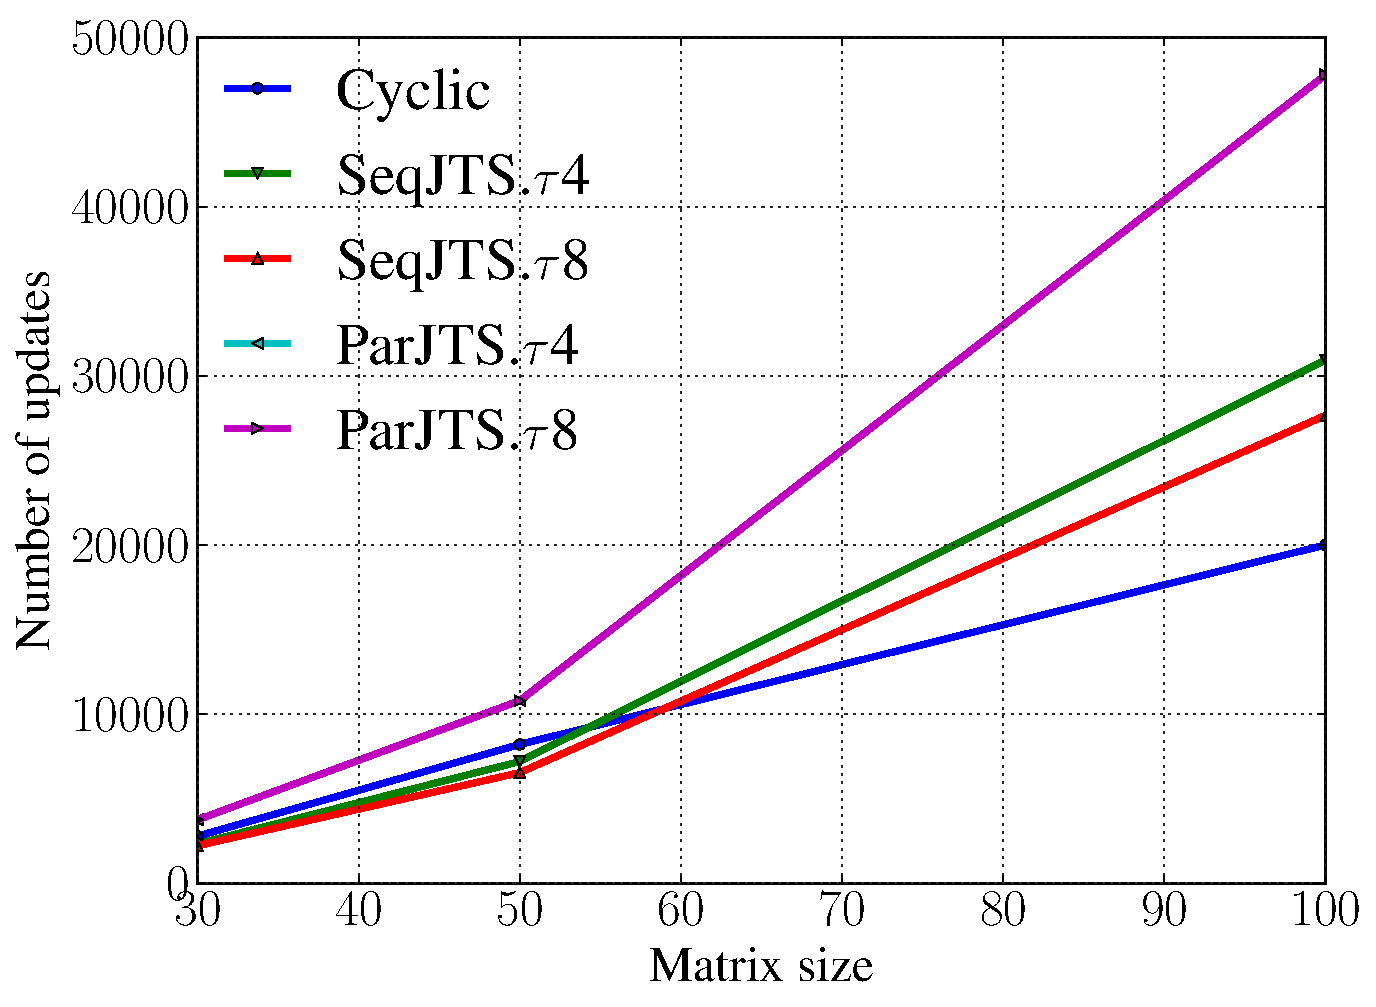
\includegraphics[width=0.48\textwidth]{updates}
 } \hfill
\subfloat[(b)][Time taken]{
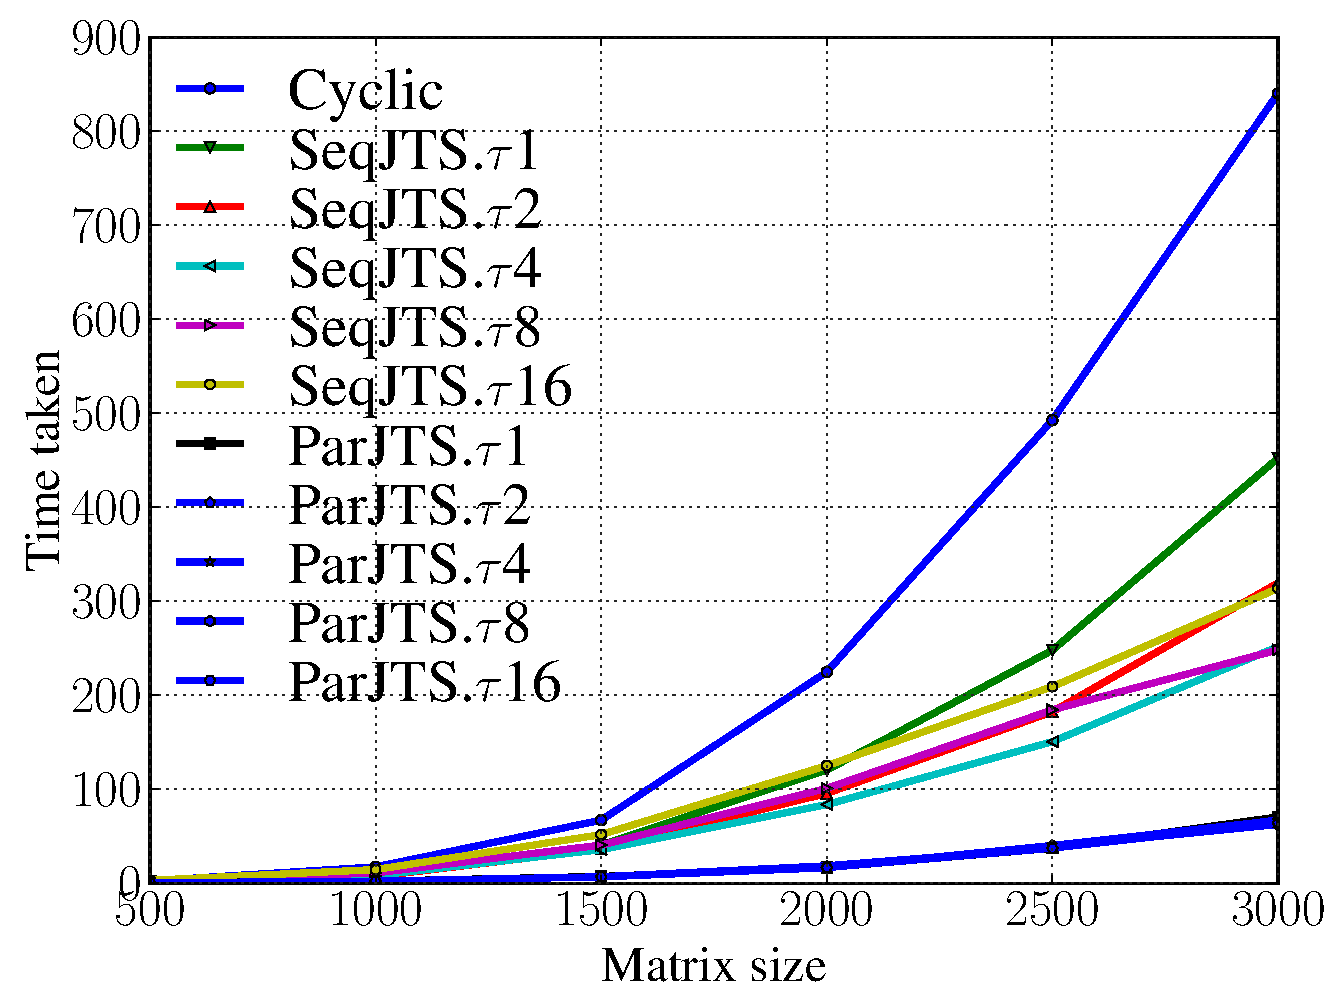
\includegraphics[width=0.48\textwidth]{timing}
 }
\caption{Performance of our parallel implementation}
\end{figure*}

\section{Conclusion}

In this paper, we have proposed a novel algorithm (called
JRS Iteration Algorithm) for computing SVDs. This algorithm
enables us to perform all the rotations in a sweep independently
and in parallel without increasing the number of sweeps
significantly. Thus this algorithm can be implemented on a
variety of parallel models of computing to obtain optimal
speedups when the processor bound is O(n 2 ). This method
significantly decreases the number of sweeps over independent
Jacobi proposed in [11]. Therefore, our method can be used
in their stream algorithm to achieve a run time of O(nS). Our
algorithm can also be implemented on a CREW PRAM to have
a run time of O(S log 2 n). In this paper we have also provided
expressions for the relaxation parameter that will result in the
minimum number of sweeps.

%% use section* for acknowledgement
%\section*{Acknowledgment}
%
%
%The authors would like to thank...
%more thanks here
%
%\begin{table}[!t]
%% increase table row spacing, adjust to taste
%\renewcommand{\arraystretch}{1.3}
% if using array.sty, it might be a good idea to tweak the value of
% \extrarowheight as needed to properly center the text within the cells
%\caption{An Example of a Table}
%\label{table_example}
%\centering
%% Some packages, such as MDW tools, offer better commands for making tables
%% than the plain LaTeX2e tabular which is used here.
%\begin{tabular}{|c||c|}
%\hline
%One & Two\\
%\hline
%Three & Four\\
%\hline
%\end{tabular}
%\end{table}


% Note that IEEE does not put floats in the very first column - or typically
% anywhere on the first page for that matter. Also, in-text middle ("here")
% positioning is not used. Most IEEE journals/conferences use top floats
% exclusively. Note that, LaTeX2e, unlike IEEE journals/conferences, places
% footnotes above bottom floats. This can be corrected via the \fnbelowfloat
% command of the stfloats package.



% trigger a \newpage just before the given reference
% number - used to balance the columns on the last page
% adjust value as needed - may need to be readjusted if
% the document is modified later
%\IEEEtriggeratref{8}
% The "triggered" command can be changed if desired:
%\IEEEtriggercmd{\enlargethispage{-5in}}

% references section

\balance

% can use a bibliography generated by BibTeX as a .bbl file
% BibTeX documentation can be easily obtained at:
% http://www.ctan.org/tex-archive/biblio/bibtex/contrib/doc/
% The IEEEtran BibTeX style support page is at:
% http://www.michaelshell.org/tex/ieeetran/bibtex/
\bibliographystyle{IEEEtran}
% argument is your BibTeX string definitions and bibliography database(s)
\bibliography{IEEEabrv,jacobi}


% that's all folks
\end{document}


